\documentclass[a4paper]{article}
\usepackage[dutch]{babel}
\usepackage{amsthm}
\usepackage{geometry}
\usepackage{answers}
\usepackage{booktabs}
\usepackage{tikz}
\usepackage{pxfonts}
\usepackage{listings}
\usepackage{framed}
\usepackage{hyperref}

\geometry{a4paper,total={210mm,297mm},left=10mm,right=10mm,top=10mm,bottom=10mm,bindingoffset=0mm}

\usetikzlibrary{shadows,calc}

\newtheoremstyle{mytheoremstyle} % name
    {1cm}                        % Space above
    {1cm}                        % Space below
    {\rmfamily}                  % Body font
    {}                           % Indent amount
    {\scshape}                   % Theorem head font
    {.}                          % Punctuation after theorem head
    {.5em}                       % Space after theorem head
    {}                           % Theorem head spec (can be left empty, meaning 'normal')

\theoremstyle{mytheoremstyle}


\Newassociation{solution}{Oplossing}{answers}
\newtheorem{Exercise}{Oefening}

\newenvironment{exercise}{\begin{center}\begin{framed}\begin{minipage}{.95\textwidth}\begin{Exercise}}{\end{Exercise}\end{minipage}\end{framed}\end{center}}



\lstset{language=SQL,basicstyle=\tt}

\tikzstyle{dbtablehead}=[]
\tikzstyle{dbtable}=[draw,drop shadow,fill=white]


\newcounter{dbtablecounter}
\makeatletter
\long\def\TABLES#1{%
  \setcounter{dbtablecounter}{0}%
  \begin{center}%
    \begin{tikzpicture}%
    #1%
    \end{tikzpicture}%
  \end{center}}
\long\def\SHOWTABLE#1#2{%
  \ifnum\value{dbtablecounter}=0%
  \@FIRSTTABLE{#1}{#2}%
  \else%
  \@NEXTTABLE{#1}{#2}%
  \fi%
  \stepcounter{dbtablecounter}%
}
\long\def\@FIRSTTABLE#1#2{
  \@FORMATTABLE{(0,0)}{#1}{#2}
}
\long\def\@NEXTTABLE#1#2{
  \addtocounter{dbtablecounter}{-1}
  \coordinate (pos) at (body\arabic{dbtablecounter}.north east);
  \addtocounter{dbtablecounter}{1}
  \@FORMATTABLE{($ (pos) + (1, 0) $)}{#1}{#2}
}
\long\def\@FORMATTABLE#1#2#3{
  \node[anchor=north west,dbtable] (body\arabic{dbtablecounter}) at #1 {#3 };
  \node[anchor=south,dbtablehead] (head\arabic{dbtablecounter}) at (body\arabic{dbtablecounter}.north) {\textsc{#2}};
}
\newcommand{\drawtable}[3]{
  \node[anchor=north west,dbtable] (body #2) at #1 {#3};
  \node[anchor=south,dbtablehead] (head #2) at (body #2.north) {\textsc{#2}};
}

\makeatother

\pagestyle{empty}


\begin{document}
% \Opensolutionfile{answers}

\begin{center}
  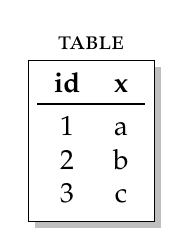
\begin{tikzpicture}
    \node[dbtable] (table) {
      \begin{tabular}{cc}
        {\bf id} & {\bf x} \\
        \toprule
        1 & a \\
        2 & b \\
        3 & c \\
      \end{tabular}
    };
    \node[dbtablehead,anchor=south] at (table.north) {\sc table};
  \end{tikzpicture}
  \hspace{5mm}
  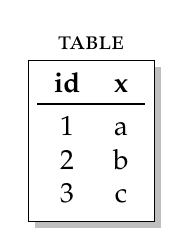
\begin{tikzpicture}
    \node[dbtable] (table) {
      \begin{tabular}{cc}
        {\bf id} & {\bf x} \\
        \toprule
        1 & a \\
        2 & b \\
        3 & c \\
      \end{tabular}
    };
    \node[dbtablehead,anchor=south] at (table.north) {\sc table};
  \end{tikzpicture}
\end{center}

% \Closesolutionfile{answers}

% \clearpage
% \section{Oplossingen}
% \begin{Oplossing}{8.1.1}
De elementen zullen van groot naar klein gesorteerd worden.
\end{Oplossing}
\begin{Oplossing}{8.1.2}
Indien de rij twee gelijke elementen bevatten, zullen deze constant verwisseld
worden en eindigt het algoritme nooit.
\end{Oplossing}
\begin{Oplossing}{8.1.3}
\inlinecode{i > 0} geeft exact hetzelfde als \inlinecode{i >= 0} vermits
\inlinecode{bubbleSortPass} nooit \inlinecode{0}
kan teruggeven: ofwel worden er geen elementen aangepast en geeft de functie \inlinecode{-1}
terug, ofwel wordt \inlinecode{i+1} teruggegeven waarbij \inlinecode{i} minimaal gelijk is aan \inlinecode{0}.
Met andere woorden, indien het element met index \inlinecode{0} wordt verplaatst, \emph{moet} ook
het element met index \inlinecode{1} zijn betrokken geweest. Vermits de index van het laatste verplaatste element
(d.i.\ dat met de hoogste index) moet teruggegeven worden, betekent dit dat \inlinecode{1} het resultaat moet zijn
(of een hogere index indien er nog andere elementen verwisseld werden).
\end{Oplossing}
\begin{Oplossing}{8.2.1}
Het resultaat blijft hetzelfde. Het geval waarbij \inlinecode{i} gelijk is aan
\inlinecode{0} komt overeen met het invoegen van een element in een lege rij.
Vermits hiervoor in ons geval niets hoeft te gebeuren, kunnen we deze stap gewoon overslaan.
In \cref{example:sorteer:insertion} kwamen we dit ook tegen: het invoegen
van 6 benodigde geen verwisselingen.
\end{Oplossing}
\begin{Oplossing}{8.2.2}
Dit doe je best niet vermits je het risico loopt om, indien \inlinecode{i == 0},
\inlinecode{rij[-1]} met \inlinecode{rij[0]} te vergelijken.
Een conjunctie (\inlinecode{&&}) wordt van links naar rechts uitgevoerd:
indien de linkervoorwaarde faalt, zal de rechtervoorwaarde niet ge\"evalueerd worden.
Eerst nakijken of \inlinecode{i-1 >= 0} verhindert dus dat \inlinecode{rij[i-1] > rij[i]}
wordt uitgevoerd indien \inlinecode{i} niet groter is dan \inlinecode{0}.

Terzijde: hoewel het gedrag
van zulke code wel gedefinieerd is in JavaScript (\inlinecode{rij[-1]} zal de waarde \inlinecode{undefined}
opleveren) en ironisch genoeg de code uiteindelijk zelfs zal werken (je kan zelfs
\inlinecode{i-1 >= 0} weglaten!), moet je JavaScript al h\'e\'el goed kennen
om op zulk gedrag te kunnen steunen teneinde correct werkende algoritmen te schrijven.
De bedoeling van deze cursus om de algoritmen te begrijpen en te kunnen implementeren,
en niet de gekheden en frivoliteiten van JavaScript te leren benutten;
indien je code steunt op zulke taalspecifieke details, zal het dan ook als fout beschouwd worden.
We willen dus dat je code weldegelijk \emph{eerst} checkt dat \inlinecode{i-1 >= 0}.
\end{Oplossing}
\begin{Oplossing}{8.2.3}
Het algoritme geeft in dit geval \inlinecode{i} terug, wat in feite foutief is.
De functie \inlinecode{selectionSort} roept echter \inlinecode{zoekIndexMinimum}
op met \inlinecode{i <= imax} waardoor alles correct werkt. In principe zou
men echter \inlinecode{zoekIndexMinimum} robuuster moeten maken.
\end{Oplossing}
\begin{Oplossing}{8.2.4}
Het geval \inlinecode{i == rij.length - 1} betekent dit dat we aan het laatste
element toe zijn. De rode rechterdeelrij bevat dus slechts \'e\'en enkel element.
Het minimum hiervan vinden is triviaal: het is dat element zelf.
We zouden dus \inlinecode{minimumIndex == i} bekomen. Vervolgens zouden we
op \cref{line:sorteer:selection:swap} die element met zichzelf verwisselen,
wat geen effect heeft. Met andere woorden, het laatste element krijgen we ``gratis'':
het staat automatisch reeds op de juiste plaats in de rij.
\end{Oplossing}
\begin{Oplossing}{8.3.1}
\inlinecode{mergeSortRec} zal zichzelf nooit oproepen met \inlinecode{begin > einde},
maar \inlinecode{mergeSort} zal echter wel \inlinecode{mergeSortRec} kunnen oproepen
met \inlinecode{begin==0} en \inlinecode{einde==-1}: dit komt voor indien
men de lege rij wil sorteren. Hoewel dit wel een randgeval is, is het belangrijk
dat dit ook correct wordt afgehandeld.
\end{Oplossing}


\end{document}
